\chapter{Sun flare detection algorithm}

Before starting to write the main solar flare detection algorithm a first program was developed in which the location of the sun was known and we knew when the solar flare had taken place.

Try algorithm knowing the location of the source, sun. Show first distribution of VTEC thtough the day (vill), then for the specific moment in time


\section{Brute force approach}





explicar aqui lo de los polos, in a first approach to this in which to visually see ourselves the differences between possible Sun positions we obtained a plot for each possibility (figure \ref{fig:poles}), we could see this happening:

\begin{figure}[!htb]
	\begin{subfigure}[b]{0.5\textwidth}
		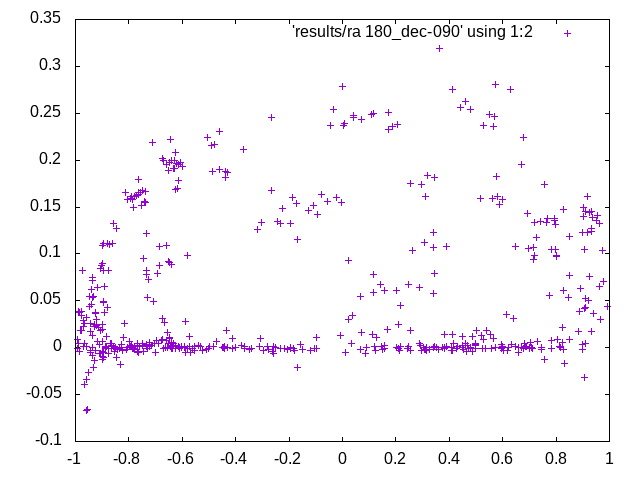
\includegraphics[width=\linewidth]{images/ch4/ra180_dec-090.png}
		\caption{ra180 and dec-090}
	\end{subfigure}
	\hfill
	\begin{subfigure}[b]{0.5\textwidth}
		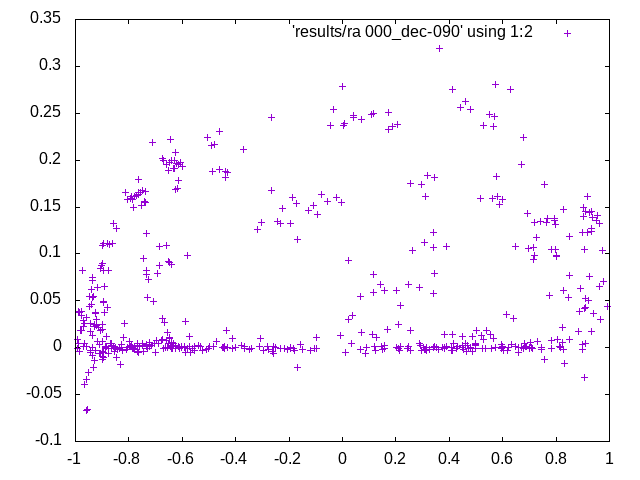
\includegraphics[width=\linewidth]{images/ch4/ra000_dec-090.png}
		\caption{ra000 and dec-090}
	\end{subfigure}
	\caption{dasdasdasda}
	\label{fig:poles}
\end{figure}

